\section{Block-Encodings}
\label{sec:block-encoding}

Quantum algorithms are constructed as a series of unitary operators.
However, it is often necessary to access information regarding non-unitary operators within a quantum algorithm.
Block-Encoding refers to an access model to non-unitary operators wherein the information regarding the operator is stored in a marked subspace of a larger unitary operator.

If we let $H$ represent some Hermitian, non-unitary operator, then a block-encoding of $H$ is given by:
\begin{equation}
    U_H = 
    \begin{pmatrix}
    \bar{H} & * \\
    * & * 
    \end{pmatrix}
\end{equation}
where $U_H$ is the larger unitary operator, $\bar{H}$ is a rescaled form of the original operator such that all matrix elements have magnitude less than one, and matrix entries $*$ denote matrix elements that are chosen such that the $U_H$ is untiary.

The action of the block-encoding on an arbitrary quantum state ($\ket{\psi}$) can be defined as:
\begin{equation}
    \ket{\psi} \ket{0}_{\text{anc}} \rightarrow_{U_H} \bar{H} \ket{\psi} \ket{0}_{\text{anc}} + \beta \ket{junk} \ket{0_\perp}_{\text{anc}}
\end{equation}
where $\ket{}_{\text{anc}}$ is the ancilla register and $\beta$ is a complex coefficient that normalizes the quantum state.
In the above equation, the encoded subspace of $\bar{H}$ is chosen (without loss of generality) to be the all-zero state of the ancilla register.
The state $\ket{junk}$ represents the state of the system register outside of the encoded subspace and can typically be disregarded.

Measurement of the ancilla after the block-encoding is apply and post-selecting on the encoded subspace gives the success probably of applying the block-encoding.
This success probability is a function of the rescaling factor of $H / \bar{H}$ and can have important implication for the cost of algorithms constructed with block-encodings.  

\subsection{Linear Combination of Unitaries}
\label{subsec:lcu}

Linear Combination of Unitary (LCU) \cite{childs2012hamiltonian} is a method for generating block-encodings of operators that can be written as:
\begin{equation}
    H = \sum_{l=0}^{L-1} \alpha_l U_l
\end{equation}
where $\alpha_l$ is some real-valued coefficient.

In this construction, the rescaled operator is given by:
\begin{equation}
    H = \lambda_{LCU} \bar{H}
\end{equation}
where the rescaling factor ($\lambda_{LCU}$) is the 1-norm of the coefficients of the unitary operators in the LCU:
\begin{equation}
    \lambda_{LCU} = \sum_{l=0}^{L-1} | \alpha_l |
\end{equation}

LCU is constructed via two oracles: \textit{Prepare} and \textit{Select}.
The action of the \textit{Prepare} oracle is to create a superposition state of an ancilla register that is weighted by the normalizes coefficients of the terms in the LCU when the ancilla register begins in the all-zero state.
We refer to this ancilla register as the \textit{index register} as it encodes the index of the term in the LCU.
This is given by:
\begin{equation}
    \ket{0^{\otimes \lceil \log_2 L \rceil}} \rightarrow_{Prepare} \sum_{l=0}^{L-1} \sqrt{| \bar{\alpha_l} |} \ket{l}
\end{equation}
where $\ket{l}$ is the computational basis state of the index register encoding the integer $l$ in binary and the noramlized coefficients are given by:
\begin{equation}
    \label{eq:asp-coeff-rescale}
    \bar{\alpha_l} = \frac{\alpha_l}{\lambda_{LCU}}
\end{equation}

The action of the \textit{Select} oracle is to apply the unitary $U_l$ onto the system register \textit{controlled} on the index regsiter being in the state $\ket{l}$.
This is given by:
\begin{equation}
    Select: 
    \begin{cases} 
        Apply \hspace{0.125cm} U_l \hspace{0.125cm} on \hspace{0.125cm} \ket{\psi} & when \hspace{0.05cm} \ket{\text{anc}} \hspace{0.05cm} is \hspace{0.05cm} \ket{l} \\
        Undefined & Otherwise \\
    \end{cases}
\end{equation}

With these two oracles defined, a block-encoding of $H$ can be realized as:
\begin{equation}
    \begin{split}
        \ket{\psi} \ket{0}_{\text{\text{index}}} &\rightarrow_{Prepare} \ket{\psi} \sum_{l=0}^{L-1} \sqrt{| \bar{\alpha_l} |} \ket{l}_{\text{\text{index}}} \\
        &\rightarrow_{Select} \sum_{l=0}^{L-1} \big(\sqrt{| \bar{\alpha_l} |} (U_l \ket{\psi}) \ket{l}_{\text{\text{index}}} \big) + \beta^* \ket{\perp^*} \\
        &\rightarrow_{Prepare^\dagger}  \bar{H} \ket{\psi} \ket{0}_{\text{\text{index}}} + \beta \ket{\perp} \\
    \end{split}
\end{equation}
where $\ket{\perp}$ and $\ket{\perp^*}$ denote quantum states of both the system and the index register that are outside the encoded subspace.
The state within the encoded subspace, $\bar{H} \ket{\psi} \ket{0}_{\text{\text{index}}}$, gives the rescaled Hamiltonian applied to the quantum state.
\ws{The math on this is a bit sketchy, particularly the junk state in the final line. Will try to find a better way to express this.}

\subsection{Sparse Block-Encoding of Pairing Hamiltonians}
\label{subsec:sparse-be}

An alternative framework for constructing block-encodings is the sparse oracle approach \cite{berry2009black, childs2009universal, lin2022lecture}.
In this approach, we assume access to two oracles: $O_A$ and $O_C$.
$O_A$ performs a controlled-rotation of a signal qubit encoding the value of the matrix element \cite{lin2022lecture}.
On inputs $\ket{l}$ and $\ket{j}$, $O_C$ returns the row index of the $l^{th}$ nonzero element in column $j$ \cite{camps2024explicit}.
The general idea of these oracles is that $O_C$ indicates where the non-zero matrix elements are and $O_A$ encodes what the values of the corresponding matrix elements are. 

In \cite{camps2024explicit}, the authors provide circuit constructions for these two oracles for certain sparse matrices.
Liu et. al \cite{liu2024efficient} use this framework to construct a sparse block-encoding for a pairing Hamiltonian of the form:
\begin{equation}
    H = \sum_{ij}h_{ij}b^\dagger_i b_j
\end{equation}

\begin{figure}[h]
    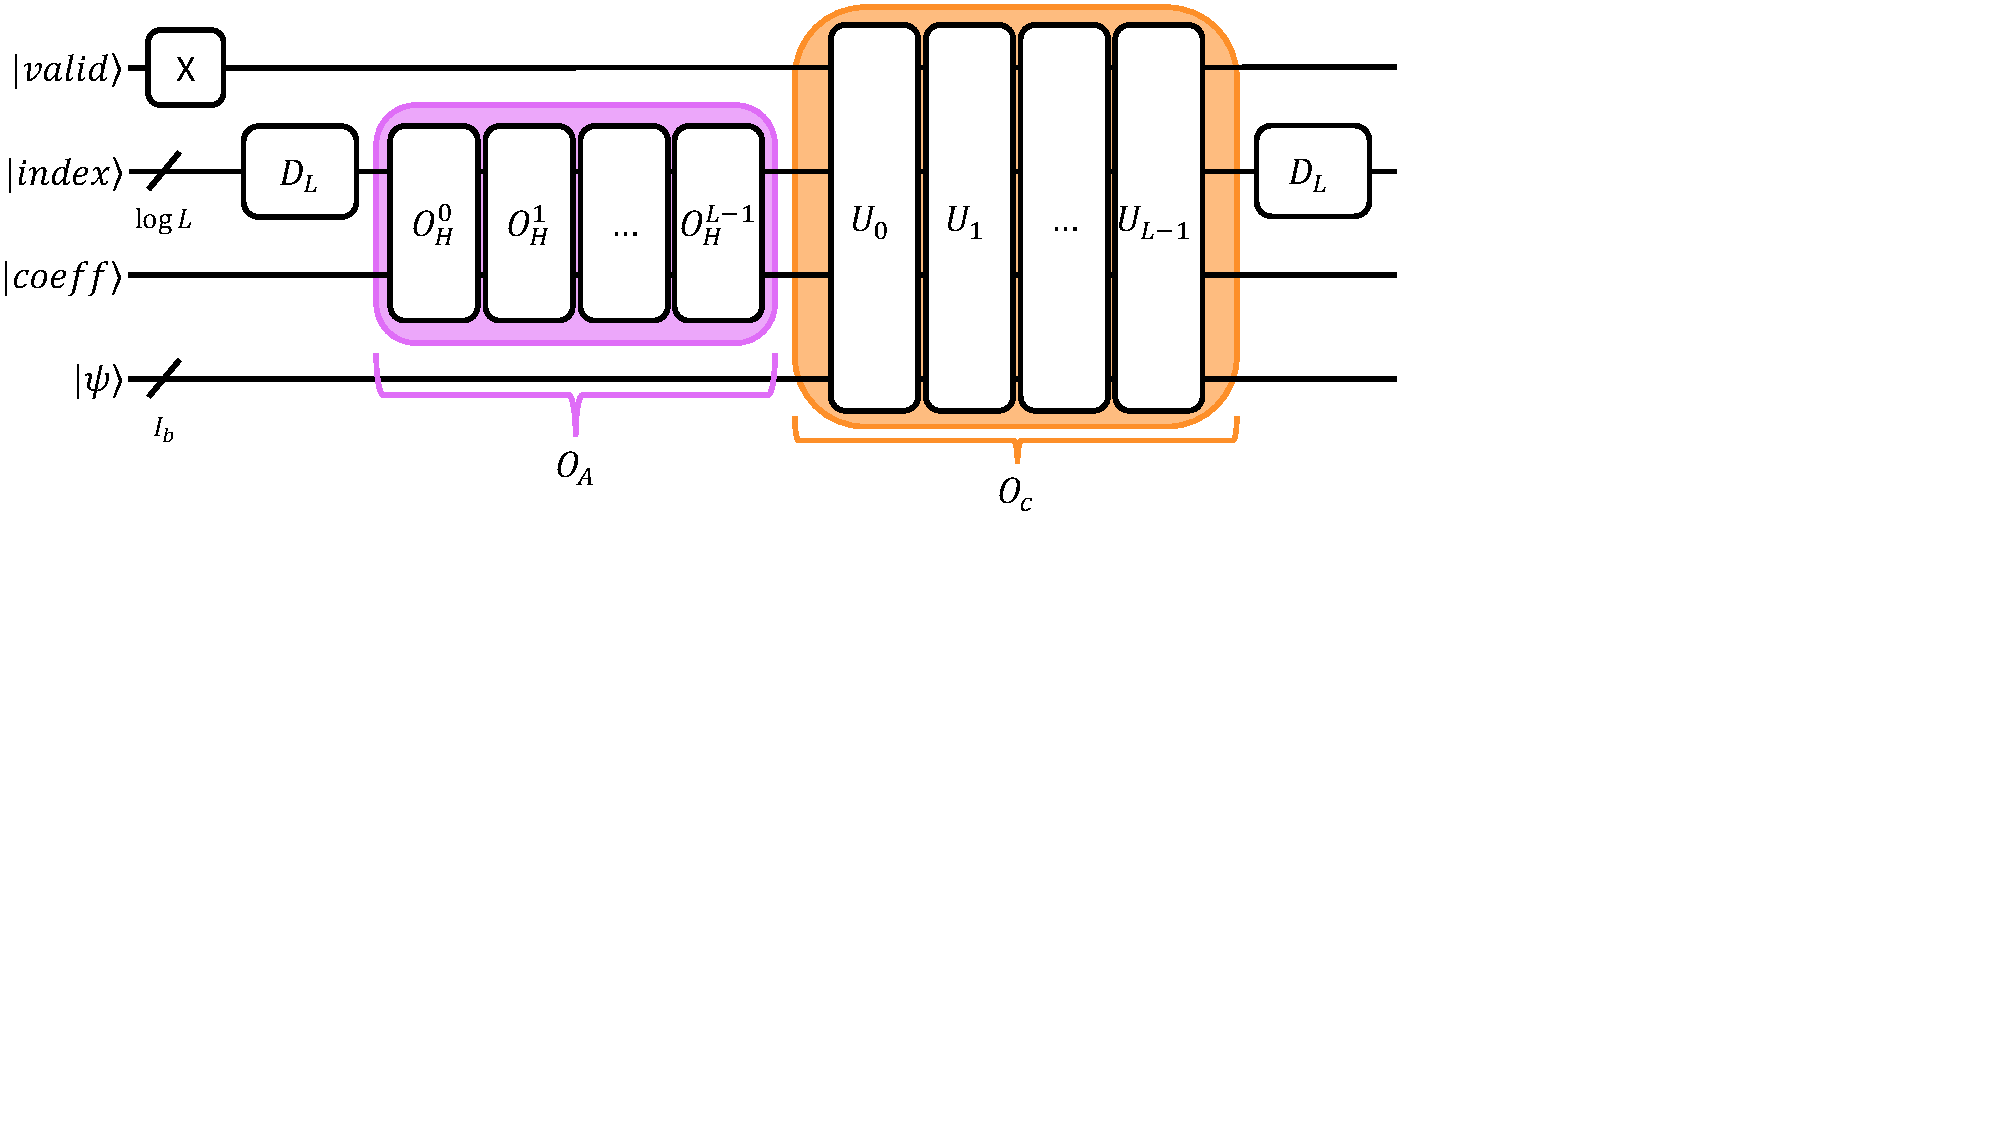
\includegraphics[width=12cm]{figures/liu-construction.pdf}
    \caption{
        \textbf{Sparse Block-Encoding Circuit for Pairing Hamiltonians}
        A circuit diagram for the block-encoding described by Liu et. al \cite{liu2024efficient} is shown.
        The \textit{Diffusion} operator is implemented via \textit{Uniform State Preparation} (USP).
        The $O_A$ oracle is implemented by the series of $O_H^l$ operators (shaded in purple) which load the coefficients of the $l^{th}$ term.
        The $O_C$ oracle is implemented by the series of $U_l$ operators (shaded in orange) which apply the $l^{th}$ term onto the state.
    }
    \label{fig:liu-construction}
\end{figure}

The layout of these circuits is given in Figure \ref{fig:liu-construction}.
The \textit{USP} oracle in Figure \ref{fig:liu-construction} represents the \textit{Diffusion} operator of \cite{camps2024explicit} and \cite{liu2024efficient}.
This oracle creates an equal superposition of basis states from $\ket{0}\dots \ket{2^{\lceil \log_2{L} \rceil} - 1}$ on the index register where $L$ is the number of terms in the Hamiltonian.
We will elaborate on this operator in Subsection \ref{subsec:prepare}.

The sequence of $O_H^l$ operators implement the $O_A$ oracle.
This oracle performs a controlled rotation on an ancilla qubit that, given the basis state from the index register, rotates the ancilla qubit proportionally to the coefficient of the term.
Explicity, this is implemented via the following steps:
\begin{algorithmic}[1]
    \For{Multiplex: $\ket{l} \in [0, L-1]$}
        \If{$\ket{\text{index}} == \ket{l}$}
            \State $\ket{\text{anc}} \gets \ket{1}$
        \EndIf

        \If{$\ket{\text{anc}} == \ket{1}$}
            \State $\theta_l \gets 2\arccos(\alpha_l)$
            \State $\ket{0}_{\text{coeff}} \gets R_y(\theta_l) \ket{0}_{\text{coeff}}$ 
        \EndIf

        \State $\ket{\text{anc}} \gets \ket{0}$
    \EndFor
\end{algorithmic}
% \begin{enumerate}
%     \item Control on the index register being in the state $\ket{l}$ and store the quantum boolean in an ancilla qubit
%     \item Controlled on this ancilla, perform a Pauli-Y rotation on an additional ancilla of the angle $\theta_l = 2\arccos(\alpha_l)$, where $\alpha_l$ is the value of $h_{ij}$ where an ordering of $i$ and $j$ gives a function: $f(i, j) = l$
%     \item The "control" qubit is then reset to $\ket{0}$
% \end{enumerate}
where the ``for'' loop is a coherent for-loop implemented by a mulitplexor over the index register.
Additionally, $\ket{\text{anc}}$ is a clean ancilla qubit and $\ket{0}_{\text{coeff}}$ is a single qubit in a ``coefficient" register that begins in the $\ket{0}$ state on the branch of the wavefunction where $\ket{\text{anc}}$ is $\ket{1}$. 
$\alpha_l$ is $h_{ij}$ and a predetermined ordering of $i$ and $j$ gives a function: $f(i, j) = l$.
A constraint on the coefficients $h_{i, j}$ is that they be scaled such that all have magnitude less than or equal to $1$ which can be easily achieved by rescaling the Hamiltonian by the maximum value of $h_{i, j}$ for all $i$ and $j$.

The $O_C$ oracle is constructed by the unitaries denoted as $U_0 \dots U_{L - 1}$. 
Each of the unitaries encodes the behavior of one term $T_l$ when acting on the system. 
In general, these unitaries are constructed with the following steps:
\begin{algorithmic}[1]
    \For{Multiplex: $\ket{l} \in [0, L-1]$}
        \If{$\ket{\text{index}} == \ket{l}$}
            \State $\ket{\text{anc}}_{\text{index}} \gets \ket{1}$
        \EndIf

        \If{$\ket{\text{anc}}_{\text{index}} == \ket{1}$ and $T_l \ket{\psi} \neq 0$ and $\ket{\text{valid}} == \ket{1}$}
            \State $\ket{\text{anc}}_{\text{ctrl}} \gets \ket{1}$
        \EndIf

        \If{$\ket{\text{anc}}_{\text{ctrl}} == \ket{1}$}
            \State $\ket{\psi} \gets T_l \ket{\psi}$
            \State $\ket{\text{valid}} \gets X \ket{\text{valid}}$
        \EndIf

        \State $\ket{\text{anc}}_{\text{ctrl}} \gets \ket{0}$
        \State $\ket{\text{anc}}_{\text{index}} \gets \ket{0}$
    \EndFor
\end{algorithmic}
% \begin{enumerate}
%     \item Control on the index register being in the state $\ket{l}$ and store the quantum boolean in an ancilla qubit
%     \item Control on the previous ancilla, the state of the subsystem that the term $T_l$ acts on nontrivially, and the validation qubit being in the state $\ket{1}$ and store the quantum boolean in an ancilla qubit. This "control" qubit now indicates if the current term should be applied onto the quantum state
%     \item A Fredkin gate swaps the occupations of the system register for $i \leftrightarrow j$. This is beecause $b^\dagger_i b_j \ket{\psi}$ is nonzero when $\ket{\psi}_i = \ket{0}$ \textit{and} $\ket{\psi}_j = \ket{1}$, in which after the term acts on $\ket{\psi}$, $\ket{\psi}_j$ and $\ket{\psi}_i$ will swap values,  \textit{or} when they are both $\ket{1}$, in which case, the operator becomes a number operator.
%     \item The "validation" qubit is set to $0$ to signify $H\ket{\psi}$ was performed.
%     \item The "control" qubit is then reset to $\ket{0}$
% \end{enumerate}
where $T_l$ in the case of the pairing Hamiltonian is performed by applying a Fredkin gate to swap occupations of the system register for $i \leftrightarrow j$.
This is because $b^\dagger_i b_j \ket{\psi}$ is nonzero when $\ket{\psi}_i = \ket{0}$ \textit{and} $\ket{\psi}_j = \ket{1}$, in which after the term acts on $\ket{\psi}$, $\ket{\psi}_j$ and $\ket{\psi}_i$ will swap values, \textit{or} when they are both $\ket{1}$, in which case, the operator becomes a number operator.
\ws{We need to clarify the bug in their construction.}

\subsection{Unification}
\label{subsec:unification}

Upon inspection of the two oracles constructed in \cite{liu2024efficient}, it can be seen that the sparse block-encoding they present can be constructed in the same framework as an LCU block-encoding, however, the terms in the linear combiation are not restricted to be unitary, but simply fermionic ladder operators.

The unitary operators comprising $O_H^l$ commute with both one another and the unitaries $U_l$. 
A more efficient ordering of these unitaries is to place $O_H^l$ directly before or after $U_l$.
In this construction, the multiplexor over the index register is only performed once and the quantum boolean determining the index can be used for both oracles:
\begin{algorithmic}[1]
    \For{Multiplex: $\ket{l} \in [0, L-1]$}
        \If{$\ket{\text{index}} == \ket{l}$}
            \State $\ket{\text{anc}}_{\text{index}} \gets \ket{1}$
        \EndIf

        \If{$\ket{\text{anc}}_{\text{index}} == \ket{1}$ and $T_l \ket{\psi} \neq 0$ and $\ket{\text{valid}} == \ket{1}$}
            \State $\ket{\text{anc}}_{\text{ctrl}} \gets \ket{1}$
        \EndIf

        \If{$\ket{\text{anc}}_{\text{ctrl}} == \ket{1}$}
            \State $\ket{\psi} \gets T_l \ket{\psi}$
            \State $\ket{\text{valid}} \gets X \ket{\text{valid}}$
        \EndIf

        \State $\ket{\text{anc}}_{\text{ctrl}} \gets \ket{0}$

        \If{$\ket{\text{anc}} == \ket{1}$}
            \State $\theta_l \gets 2\arccos(\alpha_l)$
            \State $\ket{0}_{\text{coeff}} \gets R_y(\theta_l) \ket{0}_{\text{coeff}}$ 
        \EndIf

        \State $\ket{\text{anc}}_{\text{index}} \gets \ket{0}$
    \EndFor
\end{algorithmic}
% \begin{enumerate}
%     \item Control on the index register being in the state $\ket{l}$ and store the quantum boolean in an ancilla qubit
%     \item Controlled on this ancilla, apply the term $T_l$ onto the system as described above
%     \item Controlled on this ancilla, perform a Pauli-Y rotation on an ancilla qubit of the angle $\theta_l = 2\arccos(\alpha_l)$
%     \item Uncompute the quantum boolean and proceed to the next value of $l$
% \end{enumerate}
This ordering of the oracles in the algorithm significantly reduces the number of non-Clifford operations as the multiplexor over the index register is only performed once.

One can construct a block-encoding for a Hermitian operator written as and LCU using these steps wherein $T_l$ is the $l^{th}$ unitary in the LCU.
The main difference here with the circuit construction as compared to LCU is that the \textit{Prepare} oracle is not used to load the coefficients of the terms.
Instead, the coefficients of the terms are applied to a new ``coefficient'' register one-by-one immediately after the term $T_l$ is applied on the system.

The role of the rotation on the ``coeff'' qubit is to load the coefficient by rotating the shared quantum state of the system and the ancilla register into the encoded subspace such that the amplitude in the encoded subsapce is $\sqrt{| \alpha_l |}$.
As mentioned, this serves the same effective purpose as the \textit{Prepare} oracle in LCU.
We can replace both the $O_A$ oracle and the Diffusion oracles with calls to \textit{Prepare} as is done in LCU.
This results in a block-encoding of the form:
\begin{equation}
    U_{\text{Prepare}^\dagger} \big( \prod_{l=0}^{L-1} U_l \big) U_{\text{Prepare}} \ket{\psi} \ket{0}_{\text{anc}} = \bar{H} \ket{\psi} \ket{0}_{\text{anc}} + \beta \ket{\perp}
\end{equation}
where $\big( \prod_{l=0}^{L-1} U_l \big)$ is constructed as is done in \cite{camps2024explicit,liu2024efficient}.
This series of operators applying $U_l$ implements the \textit{Select} oracle, however, instead of applying unitary operators (as is done in LCU), it applies fermionic ladder operators onto the system.

In this construction, more rotations may be required as the \textit{Prepare} oracle is called twice.
In Section \ref{sec:results} we give numerical counts for the number of rotations and often find that the number of additional rotations is not significant.
The main advantage of this construction, as opposed to the use of the Diffusion operator and $O_A$, is that the rescaling factor is often significantly smaller.
The rescaling factor in this construction is the L1-norm of the coefficients whereas the rescaling factor of the sparse-oracle implementation is $2^{\lceil \log_2{L} \rceil} * \max{\alpha_l}$ with the latter being an upper-bound of the former (Appendix \ref{sec:proof-of-rescaling-factors}).
In Subsection \ref{subsec:prepare}, these two methods and their effects on the rescaling factor are described in more detail.
In Subsection \ref{subsec:prepare}, we refer to the method using the Diffusion operator and $O_A$ as \textit{USP} and the method using the \textit{Prepare} oracle in LCU as \textit{ASP}.
